% Options for packages loaded elsewhere
\PassOptionsToPackage{unicode}{hyperref}
\PassOptionsToPackage{hyphens}{url}
\PassOptionsToPackage{dvipsnames,svgnames,x11names}{xcolor}
%
\documentclass[
  letterpaper,
  DIV=11,
  numbers=noendperiod]{scrartcl}

\usepackage{amsmath,amssymb}
\usepackage{setspace}
\usepackage{iftex}
\ifPDFTeX
  \usepackage[T1]{fontenc}
  \usepackage[utf8]{inputenc}
  \usepackage{textcomp} % provide euro and other symbols
\else % if luatex or xetex
  \usepackage{unicode-math}
  \defaultfontfeatures{Scale=MatchLowercase}
  \defaultfontfeatures[\rmfamily]{Ligatures=TeX,Scale=1}
\fi
\usepackage{lmodern}
\ifPDFTeX\else  
    % xetex/luatex font selection
  \setmainfont[]{Comfortaa}
\fi
% Use upquote if available, for straight quotes in verbatim environments
\IfFileExists{upquote.sty}{\usepackage{upquote}}{}
\IfFileExists{microtype.sty}{% use microtype if available
  \usepackage[]{microtype}
  \UseMicrotypeSet[protrusion]{basicmath} % disable protrusion for tt fonts
}{}
\makeatletter
\@ifundefined{KOMAClassName}{% if non-KOMA class
  \IfFileExists{parskip.sty}{%
    \usepackage{parskip}
  }{% else
    \setlength{\parindent}{0pt}
    \setlength{\parskip}{6pt plus 2pt minus 1pt}}
}{% if KOMA class
  \KOMAoptions{parskip=half}}
\makeatother
\usepackage{xcolor}
\usepackage[lmargin=1in,rmargin=1in,tmargin=.8in,bmargin=.8in]{geometry}
\setlength{\emergencystretch}{3em} % prevent overfull lines
\setcounter{secnumdepth}{-\maxdimen} % remove section numbering
% Make \paragraph and \subparagraph free-standing
\ifx\paragraph\undefined\else
  \let\oldparagraph\paragraph
  \renewcommand{\paragraph}[1]{\oldparagraph{#1}\mbox{}}
\fi
\ifx\subparagraph\undefined\else
  \let\oldsubparagraph\subparagraph
  \renewcommand{\subparagraph}[1]{\oldsubparagraph{#1}\mbox{}}
\fi


\providecommand{\tightlist}{%
  \setlength{\itemsep}{0pt}\setlength{\parskip}{0pt}}\usepackage{longtable,booktabs,array}
\usepackage{calc} % for calculating minipage widths
% Correct order of tables after \paragraph or \subparagraph
\usepackage{etoolbox}
\makeatletter
\patchcmd\longtable{\par}{\if@noskipsec\mbox{}\fi\par}{}{}
\makeatother
% Allow footnotes in longtable head/foot
\IfFileExists{footnotehyper.sty}{\usepackage{footnotehyper}}{\usepackage{footnote}}
\makesavenoteenv{longtable}
\usepackage{graphicx}
\makeatletter
\def\maxwidth{\ifdim\Gin@nat@width>\linewidth\linewidth\else\Gin@nat@width\fi}
\def\maxheight{\ifdim\Gin@nat@height>\textheight\textheight\else\Gin@nat@height\fi}
\makeatother
% Scale images if necessary, so that they will not overflow the page
% margins by default, and it is still possible to overwrite the defaults
% using explicit options in \includegraphics[width, height, ...]{}
\setkeys{Gin}{width=\maxwidth,height=\maxheight,keepaspectratio}
% Set default figure placement to htbp
\makeatletter
\def\fps@figure{htbp}
\makeatother

\usepackage{multicol}
\KOMAoption{captions}{tableheading}
\makeatletter
\makeatother
\makeatletter
\makeatother
\makeatletter
\@ifpackageloaded{caption}{}{\usepackage{caption}}
\AtBeginDocument{%
\ifdefined\contentsname
  \renewcommand*\contentsname{Table of contents}
\else
  \newcommand\contentsname{Table of contents}
\fi
\ifdefined\listfigurename
  \renewcommand*\listfigurename{List of Figures}
\else
  \newcommand\listfigurename{List of Figures}
\fi
\ifdefined\listtablename
  \renewcommand*\listtablename{List of Tables}
\else
  \newcommand\listtablename{List of Tables}
\fi
\ifdefined\figurename
  \renewcommand*\figurename{}
\else
  \newcommand\figurename{}
\fi
\ifdefined\tablename
  \renewcommand*\tablename{Table}
\else
  \newcommand\tablename{Table}
\fi
}
\@ifpackageloaded{float}{}{\usepackage{float}}
\floatstyle{ruled}
\@ifundefined{c@chapter}{\newfloat{codelisting}{h}{lop}}{\newfloat{codelisting}{h}{lop}[chapter]}
\floatname{codelisting}{Listing}
\newcommand*\listoflistings{\listof{codelisting}{List of Listings}}
\makeatother
\makeatletter
\@ifpackageloaded{caption}{}{\usepackage{caption}}
\@ifpackageloaded{subcaption}{}{\usepackage{subcaption}}
\makeatother
\makeatletter
\@ifpackageloaded{tcolorbox}{}{\usepackage[skins,breakable]{tcolorbox}}
\makeatother
\makeatletter
\@ifundefined{shadecolor}{\definecolor{shadecolor}{rgb}{.97, .97, .97}}
\makeatother
\makeatletter
\makeatother
\makeatletter
\makeatother
\ifLuaTeX
  \usepackage{selnolig}  % disable illegal ligatures
\fi
\IfFileExists{bookmark.sty}{\usepackage{bookmark}}{\usepackage{hyperref}}
\IfFileExists{xurl.sty}{\usepackage{xurl}}{} % add URL line breaks if available
\urlstyle{same} % disable monospaced font for URLs
\hypersetup{
  colorlinks=true,
  linkcolor={blue},
  filecolor={Maroon},
  citecolor={Blue},
  urlcolor={Blue},
  pdfcreator={LaTeX via pandoc}}

\author{}
\date{}

\begin{document}
\ifdefined\Shaded\renewenvironment{Shaded}{\begin{tcolorbox}[borderline west={3pt}{0pt}{shadecolor}, interior hidden, enhanced, frame hidden, boxrule=0pt, sharp corners, breakable]}{\end{tcolorbox}}\fi

\setstretch{1}
\begin{figure}

\begin{minipage}[t]{0.20\linewidth}

{\centering 

\caption*{Discord}

}

\end{minipage}%
%
\begin{minipage}[t]{0.05\linewidth}

{\centering 

~

}

\end{minipage}%
%
\begin{minipage}[t]{0.50\linewidth}

{\centering 

\caption*{www.gemcity.Tech}

}

\end{minipage}%
%
\begin{minipage}[t]{0.05\linewidth}

{\centering 

~

}

\end{minipage}%
%
\begin{minipage}[t]{0.20\linewidth}

{\centering 

\caption*{MeetUp}

}

\end{minipage}%
\newline
\begin{minipage}[t]{0.20\linewidth}

{\centering 

\raisebox{-\height}{


\includegraphics{../img/gemcity_discord_qr.png}

}

}

\end{minipage}%
%
\begin{minipage}[t]{0.05\linewidth}

{\centering 

~

}

\end{minipage}%
%
\begin{minipage}[t]{0.50\linewidth}

{\centering 

\raisebox{-\height}{


\includegraphics{../img/GCTSquareWhiteForeground.png}

}

}

\end{minipage}%
%
\begin{minipage}[t]{0.05\linewidth}

{\centering 

~

}

\end{minipage}%
%
\begin{minipage}[t]{0.20\linewidth}

{\centering 

\raisebox{-\height}{


\includegraphics{../img/GemCity_meetup_qr.png}

}

}

\end{minipage}%

\end{figure}

\vspace{-.25\baselineskip}

Each of our monthly user groups brings people together to explore and
learn about technology. We provide a platform for people to get
involved, exercise new skills make new friends and build a support
system.

\vspace{-.25\baselineskip}

\begin{figure}

\begin{minipage}[t]{0.60\linewidth}

{\centering 

\textbf{\Large Attend a GemCity TECH event to:}

\begin{itemize}
\tightlist
\item
  Deepen your knowledge in:

  \begin{itemize}
  \tightlist
  \item
    a technology or
  \item
    a discipline
  \end{itemize}
\item
  Grow your skills in an area
\item
  Diversify your skills
\item
  Expand your network of tech. professionals!
\item
  Find like minded people to collaborate
\item
  Share your knowledge

  \begin{itemize}
  \tightlist
  \item
    Speak at an event
  \end{itemize}
\item
  Be a part of a tech community
\end{itemize}

}

\end{minipage}%
%
\begin{minipage}[t]{0.05\linewidth}

{\centering 

~

}

\end{minipage}%
%
\begin{minipage}[t]{0.25\linewidth}

{\centering 

\vspace{-2.15\baselineskip}

\begin{longtable}[]{@{}c@{}}
\toprule\noalign{}
\endhead
\bottomrule\noalign{}
\endlastfoot

\includegraphics{../img/CodeForDayton.png} \\

\includegraphics{../img/New_To_Tech_Mascot.png} \\
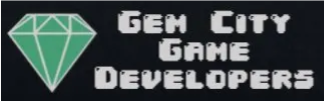
\includegraphics{../img/GemCityGameDevelopers.png} \\
\end{longtable}

}

\end{minipage}%
%
\begin{minipage}[t]{0.10\linewidth}

{\centering 

~

}

\end{minipage}%

\end{figure}

\vspace{-1.05\baselineskip}

\begin{figure}

\begin{minipage}[b]{0.05\linewidth}

{\centering 

~

}

\end{minipage}%
%
\begin{minipage}[b]{0.28\linewidth}

{\centering 


\includegraphics{../img/gem_city_ml_social.png}

}

\end{minipage}%
%
\begin{minipage}[b]{0.02\linewidth}

{\centering 

~

}

\end{minipage}%
%
\begin{minipage}[b]{0.30\linewidth}

{\centering 


\includegraphics{../img/DDLLogo.png}

}

\end{minipage}%
%
\begin{minipage}[b]{0.02\linewidth}

{\centering 

~

}

\end{minipage}%
%
\begin{minipage}[b]{0.28\linewidth}

{\centering 


\includegraphics{../img/CognitiveThinkTank.png}

}

\end{minipage}%
%
\begin{minipage}[b]{0.05\linewidth}

{\centering 

~

}

\end{minipage}%

\end{figure}

\vspace{-.5\baselineskip}

\textbf{\large Groups:}\\
Code 4 Dayton, Software Engineer, New To Tech, Cognitive Think Tank,
Dynamic Languages Group, Gem City Game Developers and GemCity Machine
Learning.

\textbf{\large Our Mission:}\\
Grow the Dayton's tech industry and community by providing a centralized
destination for training, workshops and collaborating. We are the
destination for those who are passionate about a wide range of
technology topics.

\textbf{\large Location:}\\
Downtown Dayton at the Archade / Innovation Hub. More information can be
found on MeetUp.



\end{document}
